%methods

\begin{figure*}[t]
\centering
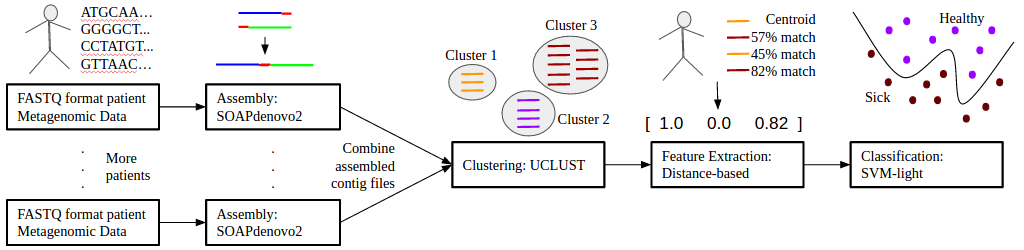
\includegraphics[scale=0.5]{./mil-metagenomics-pipeline.png}
\caption{This diagram illustrates the entire pipeline. Patient files with FASTQ metagenomic reads are individually assembled using SOAPdenovo2, then combined into one file and clustered with UCLUST. We extract features according to the D-BoW method, and classify the patients using the feature vectors with svm-light.} \label{pipeline}
\end{figure*}

\subsection{Overview}

Our proposed pipeline involves a number of steps, which serve a variety of purposes. For each patient file, we assembled the sequence reads, which served the dual purpose of generating larger contigs that contain more functional biological information and reducing the dataset size by discarding reads that could not be assembled. The clustering step assigns the contigs to certain clusters, which represent functionally similar microbes, and thus establish classes of instances that can be used as features for the classifier. We  applied our feature extraction method, which uses the D-BoW method of measuring the closest distance from a patient's reads to each cluster center. Finally, we used an SVM-based classifier to predict patient phenotype, and used several metrics to assess its accuracy. We used the SVM's decision boundary to infer information about which clusters of instances were most or least indicative of the phenotype, discussed further in the Results section. Aside from the patient labels, this process is entirely de novo, and does not consult any external databases. An illustration of this pipeline can be seen in Figure \ref{pipeline} on page \pageref{pipeline}.

\subsection{Assembly with SOAPdenovo2}

For our assembly step, we used SOAPdenovo2 \cite{luo12}, which is a de novo metagenome assembly tool. This tool was also used for assembly in the MGWAS study that our data came from. We use this method in order to compare ourselves with the MGWAS study, and because Soapdenovo2 has been proven to be one of the fastest assemblers \cite{peng12}. We tested a number of different combinations of parameters, and found that the best results came when we cut reads off after 100 base pairs (reads were 180 base pairs long originally) and used a k-mer size of 51. The average insert size was set to 350, in accordance with the reported average insert size from the MGWAS study that we used data from \cite{qin041012}. The patient files needed to be assembled separately, in order to avoid assembling reads from different patients together. Conversely, all contigs need to be in one file for clustering, to avoid inconsistent cluster assignments between different patients. Thus, we combined the contigs from each assembled patient file into a single for clustering.

\subsection{Clustering with UCLUST}

We used UCLUST \cite{Edgar10}, which has been shown to be among the simplest, fastest, and most effective clustering methods \cite{bonder090112, sun042711}. Since our contigs were not ordered, we used the usersort option, and we set the sequence match threshold to 40\%, which means that two reads needed to have 40\% of the same nucleotides to be in the same cluster. For instance, between two strings of length 100, at least 40 places in each of those strings would have to contain the same nucleotide (represented as A, T, G, or C). New contigs that did not match at least 40\% to any of the existing contigs would form the seed of a new cluster. This value of 40\% was found to be the best value based on our experiments with this dataset. Other values tried, including 50\%, 75\%, and 90\%, led to many clusters with very few reads per cluster.

\subsection{Feature Extraction}

Our feature extraction operation followed the D-BoW method. For each patient, we initialized a vector with length equal to the number of clusters. The value for each place in that patient's feature vector would then be set to the closest percentage match (0.4 to 1) of the reads from that patient to the relevant cluster seed. For instance, if there are three clusters of reads, and patient A has the cluster seed for cluster 1, no reads from cluster 2, and a read with 70\% match to cluster 3, their feature vector would be~~A = [1.0~~~0.0~~~0.7]. This is illustrated in Figure \ref{pipeline}. We implemented this feature extraction method in Python.

\subsection{Classification and Evaluation Metrics}

We performed classification with a standard SVM classifier using the generated feature vectors; in this case, we used svm-light \cite{joachims08}. The choice of classifier is not very important for D-BoW methods \cite{amores13}.


We can assess the success of our classifier in several ways. The simplest measure, accuracy, measures the percentage of instances 
that are classified correctly, represented by 
\begin{equation}
Accuracy = (TP + TN)/ (TP + TN + FP + FN)  \label{eqn:acc} 
\end{equation}
where TP, TN, FP and FN represents true positives, true negatives, false positives and false negatives respectively.

Accuracy as an evaluation metric can be biased if one of the classes 
(positive or negative)  has a larger number of examples than the other.   
Precision measures the percentage of positive predictions that 
were correct, 
whereas recall measures the percentage of positive 
examples that were correctly predicted (or retrieved). 
We can represent Precision and Recall as:

\begin{equation}
Precision = TP / (TP + FP). \label{eqn:prec}
\end{equation}
\begin{equation}
Recall = TP / (TP +FN). \label{eqn:roc}
\end{equation}

The F1 score captures the trade-offs between precision and recall in a
single metric and is the harmonic mean of precision and recall, given by:
\begin{equation}
F1-Score = 2 * (Precision * Recall)/ (Precision + Recall). \label{eqn:f1}
\end{equation}

Finally, we also use the Area Under Curve of the Receiver Operating Characteristic (AUC-ROC), which measures the performance of the classifier as the decision boundary threshold is moved. The SVM classifier generally predicts a group label to be negative if the predicted label for that group was less than 0 and predicts a group label to be positive otherwise. The AUC-ROC measures the performance of the classifier as the threshold is varied to more or less than 0. In effect, it measures how far off incorrect predictions were from being correct. AUC-ROC plots True Positive Rate versus False Positive Rate, given by:
\begin{equation}
True Positive Rate = Recall = TP / (TP + FN). \label{eqn:roc}
\end{equation}
\begin{equation}
False Positive Rate = FP / (FP + TN). \label{eqn:prec}
\end{equation}
